% !TEX root = brainscopypaste.tex
% ============================
\section{Protocol} % =========
% ============================
\label{sec:protocol}

In order to start bridging this gap, we set out to \emph{empirically} study public representation transformations at the microscopic level, aiming to stay compatible with macroscopic-level studies of these public representations.
Quotations appeared to be a perfect candidate as public representations.
First, they are usually cleanly delimited by quotation marks (and often with HTML markup in web pages), which greatly facilitates their detection in text corpora.
Second, they stem from a unique ``original'' version, and could ideally be traceable back to that version.
Third, and most importantly, their duplication should \emph{a priori} be highly faithful, apart from cases of cropping: not only should transformations be of moderate magnitude, but when specific words are not perfectly duplicated, it is safe to assume that the variation is due to involuntary cognitive bias --- as writers may expect any casual reader to easily verify, and thus criticize, the fidelity to the original quote.
Quotation evolution is therefore a perfect environment to measure cognition-induced transformations and relate those findings to macroscopic social dynamics.

\subsection{Dataset}

We relied on a reliable quotation dataset collected by \citet{Leskovec09}, large enough to lend itself to statistical analysis.
This dataset consists of the daily crawling of news stories and blog posts from around a million online sources, with an approximate publication rate of 900k texts per day, over a nine-month period of time (from August 2008 to April 2009) \cite{Leskovec09-url}.\footnote{Unfortunately, the original article~\citep{Leskovec09} does not provide additional details on the source selection methodology.}
Quotations were then automatically extracted from this corpus: each quotation is a more or less faithful excerpt of an utterance (oral or written) by the quoted person.
Quotations were then gathered in a graph and connected according to their similarity: either because they differ by very few words (in that case, no more than one word) or because they share a certain sequence of words (in that case, at least ten consecutive words).
A community detection algorithm was applied to that quotation graph to detect aggregates of tightly connected, i.e. sufficiently similar, groups of quotations (see \citet{Leskovec09} for more detail).
This analysis yielded the final data we had access to, with a total of about $70,000$ sets of quotations; each of these sets allegedly contains all variations of a same parent utterance, along with their respective publication URLs and timestamps.

\subsection{Word-level measures}

To keep the analysis palatable, we restricted the analysis to quotation transformations which consisted in the \emph{substitution} of a word by another word (and only those cases).
To quantify those substitutions, we decided to associate a number of features to each word, the variation of which we can statistically study.
The following sections detail the features we used.

\subsubsection{Standard psycholinguistic indices}

We first introduced some of the most classical psycholinguistic measures on words:

\begin{itemize}
    \item \textbf{Age of Acquisition}: the average age at which words are learned, obtained from~\citet{kuperman12},
    \item The average \textbf{Number of Phonemes} for all pronunciations of a word, obtained from the Carnegie Mellon University Pronouncing Dictionary~\citep{Weide98},\footnote{The CMU Pronouncing Dictionary is included in the NTLK package~\citep{Bird09}, the natural language processing toolkit we used for the analysis.}
    \item The average \textbf{Number of Syllables} for all pronunciations of a word, also obtained from the CMU Pronouncing Dictionary.
    \item \rk{Why exactly don't we include word frequencies as a measure?}
\end{itemize}

We also considered grammatical types within quotations by detection of \emph{Part-of-Speech} (POS) categories, using the Penn TreeBank Project typology~\citep{Santorini90} and thereby distinguishing verbs, nouns, adjectives and adverbs.
The results were however extremely similar across the various categories, exhibiting no specific effect of words belonging to different POS categories.

\subsubsection{Network-based definitions}

We rely on two types of network-based data: curated synonym associations provided by WordNet~\citep{WordNet10}, and ``free association'' relationships collected by~\citet{Nelson04}.  

The WordNet (WN) database gathers more than 117~000 concepts and about 147~000 words attached to these concepts. WordNet entries are disambiguated words, or ``\emph{lemmas}'', which are attached to concepts called ``synsets'', each of them gathering the set of lemmas corresponding to the same single meaning. Note that the choice of a synset for a lemma immediately determines the grammatical category of that lemma. Lemmas make the nodes of the semantic network (homonyms are aggregated into a single node), whose neighbors are synonymous lemmas belonging to the same synset(s) as the lemma(s) represented by that node.  In other words, synsets induce cliques in the semantic network. Links connecting two synonymous lemmas are being assigned a weight corresponding to the number of times these lemmas are mentioned by WordNet as synonyms, i.e. in the same synset. 

\rk{Explain Free Association}

\TB{The original WN network is a weighted, undirected network; the FA network is a directed network where weights have a different meaning. Both semantic networks describe synonymy relationships corresponding to qualitatively distinct forms of association: either from a linguistic viewpoint (WN) or from the perspective of actual information retrieval by humans (FA).  In  order to work in a unified framework, we consider links as an information on the existence of some sort of association between two words and transform both networks into undirected, unweighted networks.}

\bigskip
We introduce three standard network-based features, which may also be relevant psycholinguistically:
\begin{itemize}
    \item \textbf{Distance}, a classical dyadic network measure corresponding to the shortest path length between two nodes. This measure may be used as a proxy of the remoteness between two given lemmas, which is likely to have an influence on the likelihood of being a relevant substitution candidate.
    \item \textbf{Centrality} $k$, measured by the number of neighbors of a given node, and interpretable as a proxy for the polysemy of words. For the directed network FA we also define the incoming centrality $k'$ (number of neighbors pointing \emph{to} that node).  Note that in the present case, there is a quasi-perfect correlation between node degree and node \emph{PageRank} \cite{Page99}, which had already been used in \cite{Griffiths07} and may be interpreted as a generalized and recursive measure of lemma polysemy --- central nodes in the PageRank sense are those which are linked to many nodes themselves linked to many nodes, and so on, recursively.\footnote{\TB{{Betweenness coefficient}, another measure of node centrality describing the extent to which a node tends to connect otherwise remote areas of the network \cite{free:set}. More technically, it corresponds to the normalized number of shortest paths connecting dyads which pass through that node; the higher, the more important is that node in ensuring the connectedness of the rest of the network. Correlation between FA-BC and FA-PR is $0.74$; between WN-BC and WN-PR it is $0.83$.}}
    \item \textbf{Clustering coefficient} $c$, which measures the extent to which a node belongs to a local aggregate of tightly connected nodes, and defined as the ratio between the number of actual vs. possible links between a node's neighbors \cite{watt-coll}. A lemma is likely to have a higher clustering coefficient whenever the synsets to which it belongs are themselves semantically linked. This measure had been used by \citet{Chan10}.
\end{itemize}

\subsubsection{Variable correlations}

\TB{It would be difficult to discuss possible correlations between distance ($d$), on one side, and centrality ($k$ or $k'$) or clustering coefficient ($c$) on the other side, as the former is a dyadic measure while the latter are monadic measures.  We may however note that centrality and clustering are relatively weakly (and negatively) correlated, with a Pearson coefficient of $-0.26$.} \rk{remove, redundant with below}

An important question here relates to the various possible correlations between all the variables we consider.  The age of acquisition is a key variable, primarily as a usual suspect in psycholinguistic studies, and also appears to be generally correlated to all the other variables.  This coincides with an ongoing debate suggesting that age of acquisition encodes a variety of phenomena which are difficult to disentangle from more specific phenomena, which could be captured by more independent variables such as \CN.
\TB{Indeed, the minimal linear correlation of $aoa$ ($-0.31$) with other variables has a higher magnitude than the maximal linear correlation of other variables with each other ($-0.26$).} \rk{how do we get to that conclusion?}

Additionally, phonemes and syllables exhibit a strong linear correlation ($0.85$).  We see a better prediction effect of phonemes over syllables, which is consistent with \cite{nick-diss}, and choose to focus on phonemes only. \rk{check that!}

\bigskip
Network properties, finally, appear to be relatively weakly correlated with each other, across one network or between both networks (i.e. nodes with high index values are generally distinct between FA and WN), and may be used . We rely on FA as there is a direct possible psychological interpretation (that human copy-pasting may or may not show the same type of trend as human free association), noting that prediction results will be matched against WN as well. \rk{comment peut-on dire que les nœuds importants dans FA ne sont pas nécessairement importants dans WN mais que, pourtant, la forme de la prédiction est la même? cela me semble illogique en première lecture}

\begin{figure}[!th]
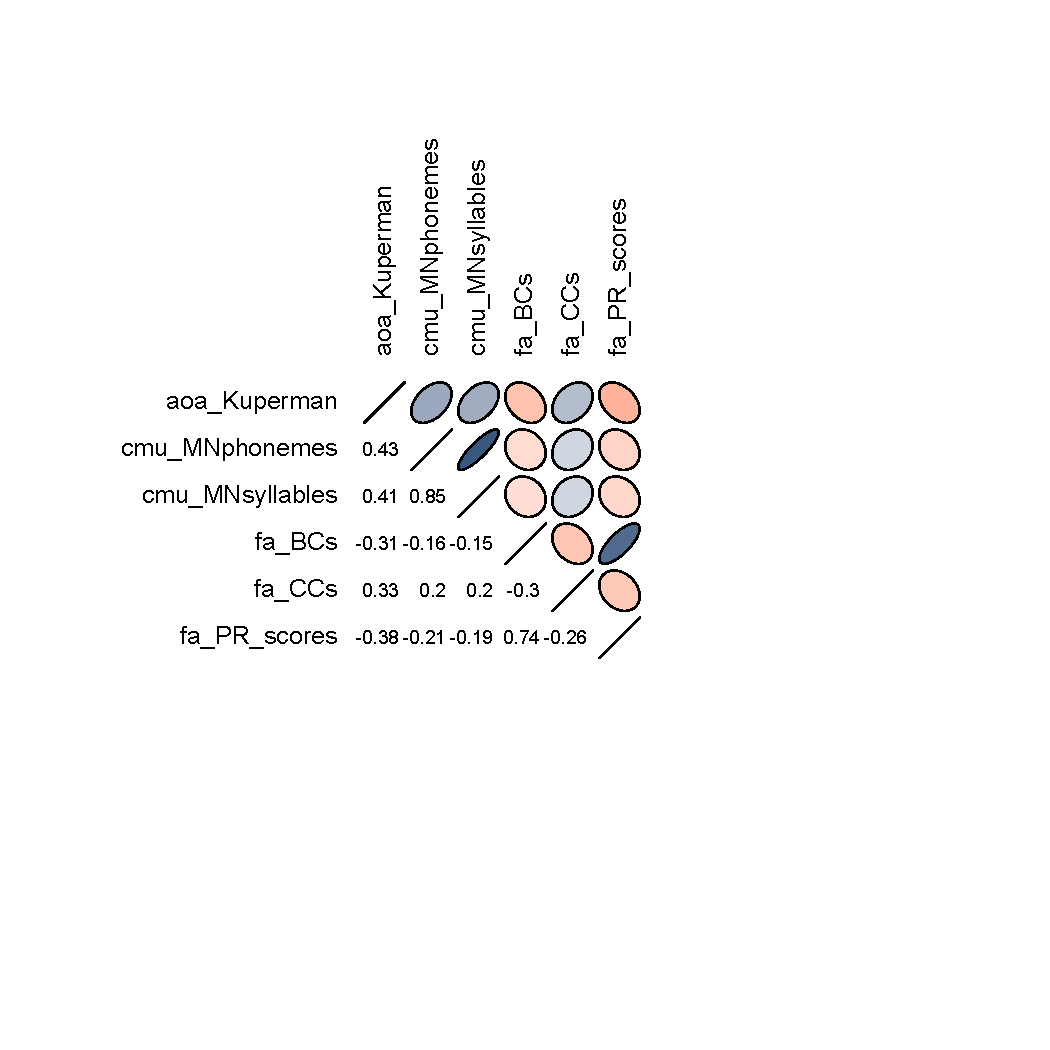
\includegraphics[width=\linewidth]{algorithms/Rplot.pdf}
\end{figure}

\subsection{Detection of substitutions}

Nonetheless, these sets bear no explicit mention of which is the authoritative, original quotation.  Defining substitutions from the dataset therefore requires additional assumptions.  
%\tb{Il manque en effet certaines informations dans le corpus pour pouvoir lire ces substitutions de façon immédiate dans les données : les métadonnées pour chaque citation ne concernant que les URLs, les dates d'apparitions et les nombres d'occurrences à chaque URL, on n'a aucune information sur les liens entre les citations. Or, on a besoin de savoir sur quelles sources un auteur s'est appuyé pour reproduire une citation, c'est-à-dire qu'on a besoin de savoir quelle citation a été générée à partir de quelle autre. Cette information n'est pas présente dans les données et on va donc devoir l'inférer, à l'aide de plusieurs hypothèses.}

Indeed, an author writing a new post and reproducing (possibly altering) a quotation bases himself on original quotations we have no access to. We face a reverse engineering problem where, given all quotations and their occurrence timestamps, we must estimate which was the originating quote for each instance of each quote. We therefore model the underlying quote selection process by making a few additional assumptions which let us define substitutions from the available data.

The main question in this problem concerns the way we consider later occurrences of a quote which, when it first appeared, was identified to be an alteration from an original quote. Let us give an example: say the quotation ``These accusations are false and absurd'' ($q_a$) appears in a blog on Jan 18th, and the slightly different quotation ``These accusations are false and incoherent'' ($q_b$) appears in another blog on the 19th, the 20th, and the 21st of January. If $q_a$ was sufficiently prominent when $q_b$ first appeared, we can safely assume that the author of $q_b$ on the 19th based himself on $q_a$. But what about the following occurrences of $q_b$? Should we consider them to be substitutions based on $q_a$ (i.e. re-creations of $q_b$ by a new instance of the substitution process that brought from $q_a$ to $q_b$ in the first place) or reproductions of the first occurrence of $q_b$?

To settle this question we model the process as follows: we assume that when a quote $q$ appears at time $t$, if not original (i.e. if not stemming from a source external to the dataset, e.g. initiating a new set of quotations), it is based solely on the most frequent quote $q_{max}$ in the preceding period of time $[t - \Delta t ; t]$. The length $\Delta t$ of that period of time is fixed as a fraction of the total duration of the considered set of quotations; we took one fifth in the implementation (i.e. one month for a set of quotations spanning five months, or one day for a set spanning only five days; this takes the dynamism of the set of quotes into account). If $q$ differs from $q_{max}$ by only a word, it is counted as a substitution from $q_{max}$ to $q$. In any other case, i.e. if $q$ and $q_{max}$ are the same or if $q$ and $q_{max}$ are different in other ways, the occurrence of $q$ is not considered to be an instance of substitution and is discarded.

An example of this detection in a situation akin to the one described above can be seen on figure \ref{fig:model-slidetimebags}: $q_a$ and $q_b$ differ by only a word, and $q_a$ appears first and stays the most frequent in the beginning. This is why the occurrences of $q_b$ at $t_1$ and $t_2$ are detected as substitutions stemming from $q_a$. After a time the situation is reversed: $q_b$ becomes more frequent than $q_a$. This entails that occurrences of $q_b$ are seen as reproductions of itself ($t_3$), and that occurrences of $q_a$ are detected as substitutions stemming from $q_b$ ($t_4$), i.e. \emph{re-creations} of $q_a$.

\begin{figure*}[h]
    \centering
    \def\svgwidth{\textwidth}
    \small
    \input{images/model-slidetimebags-b.pdf_tex}
    \caption{Detection of substitutions according to model \rk{update text in figure}}
    \label{fig:model-slidetimebags}
\end{figure*}

The assumptions embedded in this model are only a subset of a wider set of possibilities, all leading to alternative models. We identified and implemented five other such possible models, which all yielded essentially the same results. These models differ in the definition of the source quote from which new occurrences stem, essentially modifying the balance between reproduction of previous occurrences of a quote and re-creation of itself by a new substitution instance. For example, the time-windows considered can have different lengths, can include all occurrences from the beginning of the set of quotations, or can have fixed positions. The source quote of a potential substitution can be chosen among those time-windows, or otherwise (e.g. among \emph{all} quotes having appeared before $t$ and differing by a word from the considered arrival quote; this detection process would include all possible substitutions detected by other models, but would also include many false-positives).


\subsection{Characterization of substitutions}

We then measure the cognitive alteration of human copy-pasting by comparing the relative properties of substituted and substituting words in quotations.  We only consider altered quotations, \hbox{i.e.} quotations where at least one word has been modified; in other words, we measure the properties of alteration \emph{knowing that} there has been a variation (which indicates a certain reformulation) while we do not take invariant quotations into account, as it is impossible to know, in that case, whether there has been perfect individual reformulation, or just digital copy-pasting of a source (``{\sf Ctrl-C}/{\sf Ctrl-V}'').

We build two main observables for each word property. First, we measure the variation of word features over a substitution, looking at the difference of the value of a given feature between arrival and start words. %This address the question ``how do word features vary over a subs  \tb{la variation de caractéristique sémantique lors du passage du mot remplacé au mot remplaçant dans une substitution. Ceci répond à la question "comment fait-on varier la caractéristique sémantique lorsqu'on substitue un mot ?".} 
Second, we measure the susceptibility for words to be the target of a substitution, knowing that there has been a variation, in order to show which semantic features are the most likely to be the target of a substitution. % Second, \tb{la susceptibilité que les mots ont à être remplacés, en fonction de leur caractéristique sémantique. Cette mesure répond à la question "quelles caractéristiques sémantiques a-t-on plus tendance à substituer ?"%\footnote{Attention, cette mesure ne suffit pas en elle-même pour parler d'\emph{influence} de la caractéristique sémantique d'un mot sur le fait qu'il soit substitué ou non, parce qu'on n'a pas fait d'analyse des causes impliquées dans le fait qu'un mot soit substitué ; en effet, d'autres facteurs pourraient être plus importants que ces caractéristiques sémantiques dans les causes d'une substitution. On ne répond donc \emph{pas} à la question "quelle est l'influence de la caractéristique sémantique d'un mot sur sa propension à être substitué ?".}.

\subsubsection{Alteration}
%The above protocol enables us to observe in detail how word features vary upon substitution. 
For a given feature $\mathfrak{F}$, we measure how a word $\wstart$'s feature varies as $\wstart$ is substituted by $\warrival$. Let us denote this quantity:
$$\Delta (\wstart,\warrival) \defeq \mathfrak{F}(\warrival) - \mathfrak{F}(\wstart)$$

Averaging this value over all start words with a given feature value $f$ yields the mean variation for that feature value $f$.\footnote{To avoid any auto-correlation effect due to the number of substitutions in a cluster, we first average substitutions over each cluster, by considering the average of arrival word features for a given starting word. Indeed, substitutions occurring in the same cluster are likely not statistically independent.} This 
quantity can be written:
$$\left< \Delta(\wstart,\warrival) \right>_f = \left< \mathfrak{F}(\warrival) - \mathfrak{F}(\wstart) \right>_{\left\lbrace (\wstart,\warrival) | \mathfrak{F}(\wstart) = f \right\rbrace}$$

We introduce a null hypothesis $\mathcal{H}_0$ to compare the actual variation of a word's feature to its expected variation assuming the arrival word $\warrival_{\mathcal{H}_0}$ had been chosen randomly from % , let us denote the corresponding quantity This value is to be compared to the variation the word's feature would have undergone had the arrival word been chosen randomly in 
the pool of \TB{WN/FA} words. The corresponding average quantity over all start words may be written as:\footnote{Note that $\warrival_{\mathcal{H}_0}$ is in fact constant in this averaging, since by definition it does not depend on $\wstart$.}
%$$\Delta_{\mathcal{H}_0} (\wstart,\warrival) \defeq f\left(\warrival_{\mathcal{H}_0}\right) - f\left(\wstart\right)$$
%and, similarly, we compute the average over all start words 
$$\left< \Delta(\wstart,\warrival_{\mathcal{H}_0}) \right>_f
= \left< \mathfrak{F}({\warrival_{\mathcal{H}_0}}) - \mathfrak{F}(\wstart) \right>_{\left\lbrace (\wstart,\warrival_{\mathcal{H}_0}) | \mathfrak{F}(\wstart) = f \right\rbrace}$$
%Averaging over all start words with a given feature value $f$, we get $$\left< \Delta_{\mathcal{H}_0} \right>_f = \left< \mathfrak{F}({\warrival_{\mathcal{H}_0}}) - \mathfrak{F}(\wstart) \right>_{\left\lbrace \wstart | \mathfrak{F}(\wstart) = f \right\rbrace}$$

We also considered an alternative null hypothesis, denoted $\mathcal{H}_{00}$, where the arrival word is chosen randomly \emph{among immediate synonyms of the start word} (neighbors), i.e. an arrival word chosen among semantically plausible though still random words (in this case $\warrival_{\mathcal{H}_{00}}$ does depend on $\wstart$). %The values for $d$ were decided upon according to the distribution of distances travelled on the synonym graph upon substitution, normalized by the number of synonyms at that distance. 
%  brought all variation curves shown below nearer to the origin, but did not change the results qualitatively.
%The variation of feature compared to $\mathcal{H}_0$ is then $\left< \Delta \right>_f - \left< \Delta_{\mathcal{H}_0} \right>_f$.

Using this method we obtain the mean variation of feature for each start feature value, and can compare the variations to a situation where arrival words are chosen randomly. This gives us a fine-grained view of how word features evolve upon substitution.


\subsubsection{Susceptibility}


Furthermore, the protocol lets us compute substitution \emph{susceptibilities} for each feature value $f$. 
We say that a word is \emph{substitutable} if it appears in a quote which undergoes a substitution, whether that substitution operates on the considered word or on another. 
Word substitution susceptibility (denoted $\mathfrak{S}_{\mathfrak{F}}(w)$) is computed as the ratio of the number of times $n_s(w)$ a word is substituted to the number of times $n_p(w)$ that word appears in a substitutable position.  We have:
$$\mathfrak{S}_{\mathfrak{F}}(w) \defeq \frac{n_s(w)}{n_p(w)}$$

Now averaging over all words having a given feature value $f$, we obtain the mean susceptibility for the feature value $f$:
$$\left< \mathfrak{S}_{\mathfrak{F}} \right>_f = \left< \frac{n_s(w)}{n_p(w)} \right>_{\left\lbrace w | \mathfrak{F}(w) = f \right\rbrace}$$

This measure focuses on the selection of start word instead of the selection of the arrival word. Indeed, the features have an effect not only on the choice of a new word when a substitution takes place, but also at the preceding moment when it is not yet known which word in the quote --~if any~-- will be substituted. 


